\section{Context}
This thesis is the product of the participation of a team of students to a robotic contest named RoboCup.

This contest is divided into several leagues :
\begin{itemize}
\item RoboCup Soccer : historically the first category, centered about robots playing football in small teams. 
\item RoboCup Industrial : a category for more industrially focused contests.
\item RoboCup@Home : a league for domestic robots that support elder people and stuff.
\item RoboCupJunior : more of an iniative that aims to foster robotics interest in children, it helps organize various events for younger minds.
\end{itemize}
The ultimate goal of Robocup is to create a team of robots able to beat human champions in football by 2050, as illustrated by the following quote :
\begin{quote}
By the middle of the 21st century, a team of fully autonomous humanoid robot soccer players shall win a soccer game, complying with the official rules of FIFA, against the winner of the most recent World Cup.
\end{quote}

Our team will participle in the kidsize category of the humanoid part of the contest. This means we will have to build a humanoid robot, for the first time at the Montefiore Institute.

\begin{figure}[htp]
\center
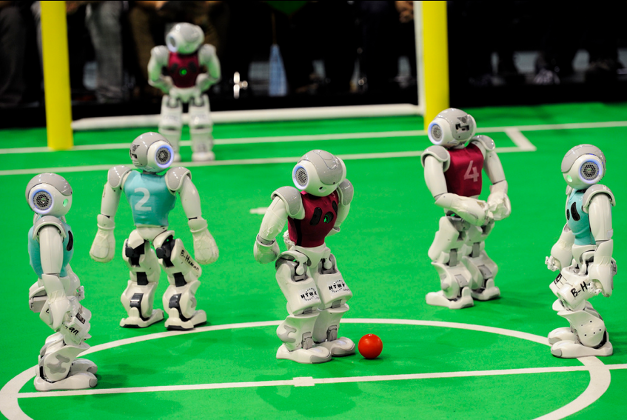
\includegraphics[width=0.5\textwidth]{figures/robocup}
\caption[Two teams of Nao robots playing against each other]{Two teams of Nao robots playing against each other in the 2014 edition of RoboCup \textit{[Photo courtesy of RoboCup]}}
\label{fig:intro_robocup}
\end{figure}

We thus need a reliable simulation tool to :
\begin{enumerate}
\item Test different robot designs and choose the best one, without spending time building a robot in real-life.
\item At a later stage, be able to test control algorithms faster because the real robot is not needed.
\end{enumerate}

\section{Goals of the project}
The goal of this thesis is to provide the team with a simulation tool and a model able of :
\begin{itemize}
\item realistically simulating the dynamics of the robot including springs and dampers
\item receiving orders at approximately 300Hz, and we don't really care if the simulation is not in real time.
\item the simulated robot receives exactly the same orders as the real robot would.
\item visualization
\end{itemize}
As the robot is still being designed this thesis should give some insights on how to build it.

\section{Structure of the report}
The report will begin with an overview of the available simulation tools and a choice for this project.

The next chapter will detail the chosen tools. The third chapter will be about tuning and verifying the accurateness of the simulation.

The fourth chapter will show some simulation examples and explain how they influence the design of the robot.

The last chapter will be the conclusion where the work will be summed up and future work prospects laid out.